\documentclass[11pt,a4paper]{hwz-thesis}

\usepackage[german,ngerman]{babel}
\usepackage[a4paper,portrait,twoside,inner=3.25cm,outer=3.5cm,top=3.5cm,bottom=4.0cm]{geometry}
% xcolor must be loaded here, else definecolor warnings show up
\usepackage{xcolor}
\usepackage{hwz}

\hypersetup{
    pdftitle = HWZ Thesis Example,
    pdfauthor = Ivan Wolf,
    pdfsubject = Example for the HWZ Thesis LaTeX style,
    pdfkeywords = example,
    colorlinks = true,
    linkcolor = blue,%red,
    anchorcolor = blue,%red,
    citecolor = black,%blue,
    filecolor = black,%red,
    urlcolor = blue,%red,
    plainpages = false,
    bookmarksnumbered = true
} 

\title{Der Titel}
\subtitle{Hat nat�rlich auch einen Untertitel}
\category{Bachelor Thesis}
\author{Ivan Wolf}
\email{$<$ivan.wolf@student.fhhwz.ch$>$}
\professor{Prof. Dr. Walter Kuhn}
\assistant{}
\school{HWZ Hochschule f�r Wirtschaft}
\department{Z�rcher Fachhochschule}
\version{}
\date{\today}
\copyrightyear{2005}

\makeindex
\makeglossaries

%A
\begin{comment}
%==> dit is het woord waarnaar verwezen wordt in de tekst
\newglossaryentry{}{
%==> dit is hetgene dat wordt getoond in de glossaries lijst
name={},
%==> dit is de beschrijving van de glossary
description={}
}

%==> dit is het woord waarnaar verwezen wordt in de tekst
\newglossaryentry{}{
%==> dit is hetgene dat wordt getoond in de glossaries lijst
name={},
%==> dit is de beschrijving van de glossary
description={}
}

%==> dit is het woord waarnaar verwezen wordt in de tekst
\newglossaryentry{}{
%==> dit is hetgene dat wordt getoond in de glossaries lijst
name={},
%==> dit is de beschrijving van de glossary
description={}
}

%==> dit is het woord waarnaar verwezen wordt in de tekst
\newglossaryentry{}{
%==> dit is hetgene dat wordt getoond in de glossaries lijst
name={},
%==> dit is de beschrijving van de glossary
description={}
}

%==> dit is het woord waarnaar verwezen wordt in de tekst
\newglossaryentry{}{
%==> dit is hetgene dat wordt getoond in de glossaries lijst
name={},
%==> dit is de beschrijving van de glossary
description={}
}


\end{comment}

\newglossaryentry{accesscontrollist}{
name={Access Control List },
description={ }
}


%% The actual document
%% ---------------------------------------------------------------------------------------------
\begin{document}

	\frontmatter

% Titelseite
% @todo Oben auf der zweiten Seite des Titelblatts weitere Angaben (About the Author, Bild? :-), Adresse, Studiengruppe, ...)
\maketitlepage

% Management Summary
\abstract{Management Summary}{chapters/abstract}

% Inhaltsverzeichnis
\toc

% Vorwort
\preface{Vorwort}{chapters/preface}

	\mainmatter

% The main content
% !Mode:: "TeX:UTF-8"
\chapter{绪论}
我是绪论中的正文文本。

\section{课题背景}
我要使用引用命令为我的文章引用文献:
\ldots~加速度为~\SI{12345}{\square\micro\meter\per\nano\second},是一般加速度的\num{1.2345e3}倍~\supercite{Yablonovitch1987},误差~\SI{+-2e-6}{\square\micro\meter\per\nano\second}。

\subsection{该小节插图}
这里我要使用图形环境插图。注意该插图拥有中英双语图注和自动生成的图形编号。同时我要引用该图形:该图的编号是~\ref{fig-pcf}。
\begin{figure}[hptb]
 \centering
 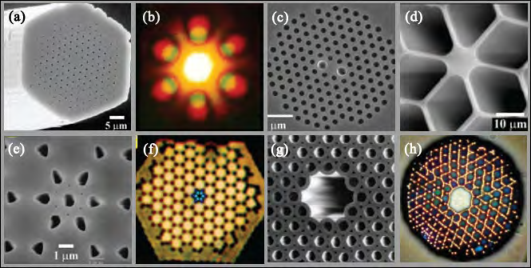
\includegraphics{chp-1_pcf}
 \caption{形式多样的光子晶体光纤。} \label{fig-pcf}
\end{figure}

\subsection{该小节插入公式}
我还要使用公式环境插入公式。注意公式是自动居中编号。同时我也要引用该公式,该公式的编号是~\eqref{equ-sample}
\begin{equation}\label{equ-sample}
\sum_{i=1}^n\sin\beta_i^2+\int_a^b\frac{D}{c}\,\mathrm{d}x=0
\end{equation}

\section{本章小结}
以上为本章的所有内容。

	\appendix

% Anhang
%%%%%%%%%%%%%%%%%%%%% appendix.tex %%%%%%%%%%%%%%%%%%%%%%%%%%%%%%%%%
%
% sample appendix
%
% Use this file as a template for your own input.
%
%%%%%%%%%%%%%%%%%%%%%%%% Springer-Verlag %%%%%%%%%%%%%%%%%%%%%%%%%%

\chapter{Chapter Heading}
\label{introA} % Always give a unique label
% use \chaptermark{}
% to alter or adjust the chapter heading in the running head

Use the template \emph{appendix.tex} together with the Springer document class SVMono (monograph-type books) or SVMult (edited books) to style appendix of your book in the Springer layout.


\section{Section Heading}
\label{sec:A1}
% Always give a unique label
% and use \ref{<label>} for cross-references
% and \cite{<label>} for bibliographic references
% use \sectionmark{}
% to alter or adjust the section heading in the running head
Instead of simply listing headings of different levels we recommend to let every heading be followed by at least a short passage of text. Further on please use the \LaTeX\ automatism for all your cross-references and citations.


\subsection{Subsection Heading}
\label{sec:A2}
Instead of simply listing headings of different levels we recommend to let every heading be followed by at least a short passage of text. Further on please use the \LaTeX\ automatism for all your cross-references and citations as has already been described in Sect.~\ref{sec:A1}.

For multiline equations we recommend to use the \verb|eqnarray| environment.
\begin{eqnarray}
\vec{a}\times\vec{b}=\vec{c} \nonumber\\
\vec{a}\times\vec{b}=\vec{c}
\label{eq:A01}
\end{eqnarray}

\subsubsection{Subsubsection Heading}
Instead of simply listing headings of different levels we recommend to let every heading be followed by at least a short passage of text. Further on please use the \LaTeX\ automatism for all your cross-references and citations as has already been described in Sect.~\ref{sec:A2}.

Please note that the first line of text that follows a heading is not indented, whereas the first lines of all subsequent paragraphs are.

% For figures use
%
\begin{figure}[t]
\sidecaption[t]
% Use the relevant command for your figure-insertion program
% to insert the figure file.
% For example, with the graphicx style use
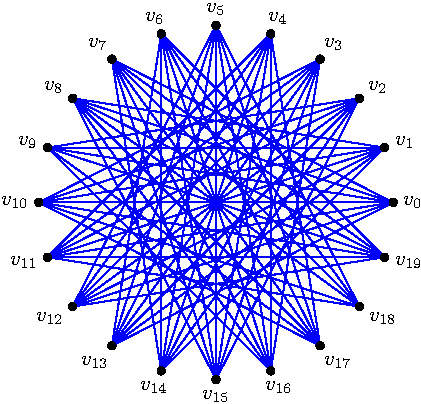
\includegraphics[scale=.65]{figure}
%
% If no graphics program available, insert a blank space i.e. use
%\picplace{5cm}{2cm} % Give the correct figure height and width in cm
%
\caption{Please write your figure caption here}
\label{fig:A1}       % Give a unique label
\end{figure}

% For tables use
%
\begin{table}
\caption{Please write your table caption here}
\label{tab:A1}       % Give a unique label
%
% Follow this input for your own table layout
%
\begin{tabular}{p{2cm}p{2.4cm}p{2cm}p{4.9cm}}
\hline\noalign{\smallskip}
Classes & Subclass & Length & Action Mechanism  \\
\noalign{\smallskip}\hline\noalign{\smallskip}
Translation & mRNA$^a$  & 22 (19--25) & Translation repression, mRNA cleavage\\
Translation & mRNA cleavage & 21 & mRNA cleavage\\
Translation & mRNA  & 21--22 & mRNA cleavage\\
Translation & mRNA  & 24--26 & Histone and DNA Modification\\
\noalign{\smallskip}\hline\noalign{\smallskip}
\end{tabular}
$^a$ Table foot note (with superscript)
\end{table}
%


% Bibliography
\showbibliography{authordate1}{hwz}

% Abbildungs- und Tabellenverzeichnis
\listoffigures
\listoftables

% Glossary
\showglossaries

% Index
\showindex

% Insert an empty page at the end
\theend

% @todo Ehrenw�rtliche Erkl�rung
	
\end{document}